\documentclass[12pt]{article}
\usepackage[utf8]{inputenc}
\usepackage[brazil]{babel}
\usepackage{amsmath, amsgen, amstext, amsbsy, amsopn, amsfonts, hyperref,  url, graphicx, tabularx, array, geometry, color}

\pagestyle{plain}


\setlength{\parskip}{1ex}
\setlength{\parindent}{0pt}

\renewcommand{\title}[1]{\textbf{#1}\\}
\renewcommand{\line}{\begin{tabularx}{\textwidth}{X>{\raggedleft}X}\hline\\\end{tabularx}\\[-0.5cm]}
\newcommand{\leftright}[2]{\begin{tabularx}{\textwidth}{X>{\raggedleft}X}#1%
& #2\\\end{tabularx}\\[-0.5cm]}


\begin{document}

\title{Oficina de Processing [at] Tarrafa Hackerspace}
\line
\leftright{\today}{Lucas Tonussi}

\section{Cor}

\qquad Temos também um suporte incrível a coloração em processing, atendendo a gostos diferentes de modos de trabalho. Para entender RGB Color basta se lembrar de quando você estava no primário e a tia Cássia dava como tarefa misturar as cores com os dedos e ver no que dava.

\qquad Diagrama de Venn:
\begin{center}
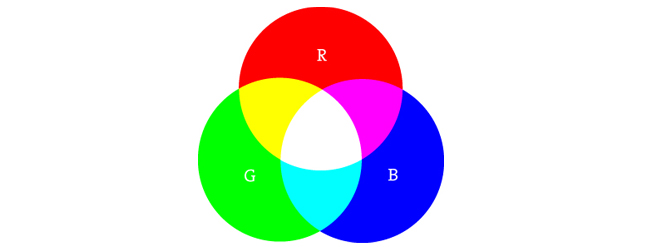
\includegraphics[scale=0.45]{rgb}
\end{center}

\begin{itemize}
\item Vermelho + Verde = Amarelo
\item Vermelho + Azul = Rosa
\item Verde + Azul = Azul Esverdeado
\item Vermelho + Verde + Azul = Branco
\item Sem cores = Preto
\end{itemize}

\subsection{Estudo da coloração}

\qquad

Cor:
\begin{itemize}
\item background()
\begin{itemize}
\item background(VALOR, VALOR, VALOR, ALPHA)
\end{itemize}
\item colorMode()
\begin{itemize}
\item colorMode(MODO, COMPRIMENTO, COMPRIMENTO, COMPRIMENTO);
\end{itemize}
\item stroke()
\begin{itemize}
\item stroke(VALOR, VALOR, VALOR, ALPHA)
\end{itemize}
\item fill()
\begin{itemize}
\item fill(VALOR, VALOR, VALOR, ALPHA)
\end{itemize}
\item tint()
\begin{itemize}
\item tint(VALOR, VALOR, VALOR, ALPHA)
\end{itemize}
\item noFill()
\item noStroke()
\item noTint()
\end{itemize}

\subsection{Exercício 1}

\begin{verbatim}
noStroke();
colorMode(HSB, 100);
for (int i = 0; i < 100; i++) {
  for (int j = 0; j < 100; j++) {
    stroke(i, j, 100);
    point(i, j);
  }
}
\end{verbatim}

\subsection{Exercício 2}

\begin{verbatim}
noStroke();
colorMode(RGB, 100);
for (int i = 0; i < 100; i++) {
  for (int j = 0; j < 100; j++) {
    stroke(i, j, 0);
    point(i, j);
  }
}
\end{verbatim}

\subsection{Exercício 3}

\qquad Nesse exercício e no código abaixo foi feito um exemplo de Saturação misturando um pouco o que aprendemos no primeiro em \textbf{oficina-processing-00}. A A Saturação é o quanto a cor é intensa ou não e representa a quantidade de escala cincenta. Ou seja, uma cor saturada diz-se uma cor pura e uma cor insaturada tem grau de escala cinzenta (porcentagem). O que é bastante interessante trabalhar.

\begin{verbatim}
int barWidth = 5;
int lastBar = -1;


void setup() {
  size(200, 200);
  colorMode(HSB, width, height, 100);
  noStroke();
}


void draw() {
  int whichBar = mouseX / barWidth;
  if (whichBar != lastBar) {
    int barX = whichBar * barWidth;
    fill(barX, mouseY, 66);
    rect(barX, 0, barWidth, height);
    lastBar = whichBar;
  }
}
\end{verbatim}

\subsection{Exercício 4}

\begin{verbatim}
PImage b;
b = loadImage("tarrafa.png");
image(b, 0, 0);
tint(0, 153, 204);
image(b, 50, 0);
\end{verbatim}

\end{document}
